\chapter{Phương pháp đề xuất}
\label{Chapter3}

\section{Phân loại zero-shot với BioMedCLIP và định hướng cải tiến}
\label{sec:ch3_biomedclip_baseline}

Với việc được tiền huấn luyện trên PMC-15M, một tập dữ liệu y sinh quy mô lớn có bao gồm ảnh X-quang, BioMedCLIP \cite{BiomedCLIP} được lựa chọn làm mô hình nền tảng để phát triển hệ thống phân loại. Trước khi xây dựng phương pháp đề xuất, nhóm khảo sát khả năng chuyển trực tiếp tri thức của mô hình sang bài toán phân loại ảnh X-quang xương trong thiết lập \textit{suy luận không mẫu}. Khảo sát này giúp làm rõ cơ chế phân loại ban đầu của BioMedCLIP và xác định những khía cạnh cần thích nghi với dữ liệu đích.

Phần này tập trung mô tả quy trình phân loại và các định hướng cải tiến. Thiết kế thực nghiệm được trình bày tại Mục \ref{sec:experiment_content}, còn kết quả định lượng và phần bàn luận tương ứng được trình bày tại Mục \ref{subsec:foundation_model_evaluation} của Chương 4 để tránh lặp lại nội dung thực nghiệm trong chương phương pháp.

\subsection{Quá trình phân loại của BioMedCLIP}
\label{subsec:ch3_biomedclip_classification}

BioMedCLIP trong thiết lập \textit{không mẫu} thực hiện phân loại dựa trên cơ chế đối sánh ảnh-văn bản thay vì sử dụng một đầu phân loại được huấn luyện trên dữ liệu đích. Quy trình gồm năm bước chính:

\begin{enumerate}
    \item \textbf{Xây dựng câu nhắc văn bản:} Với mỗi lớp, tên bệnh lý được đưa vào một câu nhắc mô tả ảnh X-quang, chẳng hạn \texttt{A radiograph showing osteosarcoma.} đối với lớp sarcoma xương. Cùng một mẫu câu được áp dụng nhất quán cho toàn bộ tập lớp.
    \item \textbf{Trích xuất đặc trưng văn bản:} Câu nhắc của từng lớp được đưa qua nhánh mã hóa văn bản sử dụng kiến trúc PubMedBERT để tạo các vectơ đặc trưng lớp trong không gian biểu diễn chung.
    \item \textbf{Trích xuất đặc trưng hình ảnh:} Ảnh X-quang đầu vào được xử lý qua nhánh mã hóa thị giác sử dụng kiến trúc Vision Transformer để tạo vectơ đặc trưng đại diện cho thông tin thị giác.
    \item \textbf{Tính độ tương đồng:} Độ tương đồng côsin được tính giữa vectơ ảnh và vectơ văn bản của từng lớp. Cặp ảnh - văn bản có sự tương hợp cao nhất về mặt ngữ nghĩa y khoa sẽ đạt điểm số lớn nhất.
    \item \textbf{Đưa ra dự đoán:} Các điểm số tương đồng được chuẩn hóa thông qua hàm Softmax để chuyển thành phân phối xác suất. Lớp tương ứng với câu mô tả có xác suất cao nhất sẽ được lựa chọn làm kết quả dự đoán của mô hình.
\end{enumerate}

\subsection{Định hướng cải tiến}
\label{subsec:ch3_improvement_directions}

Các kết quả và phân tích ở Chương 4 cho thấy mô hình nền tảng có khả năng phân biệt ban đầu nhưng chưa thể áp dụng trực tiếp cho bài toán đích. Từ những hạn chế đó, nghiên cứu đề xuất các cải tiến sau:

\textbf{Tinh chỉnh với dữ liệu hạn chế:} LoRA được lựa chọn vì đây là phương pháp tinh chỉnh hiệu quả về tham số, cho phép thích nghi BioMedCLIP với miền ảnh X-quang xương mà vẫn bảo toàn phần lớn tri thức tiền huấn luyện. So với tinh chỉnh toàn bộ tham số, LoRA giúp giảm số tham số cần cập nhật và hạn chế nguy cơ quá khớp trong bối cảnh dữ liệu y khoa có quy mô hạn chế, phân bố lớp không đồng đều. Mặc dù nghiên cứu sử dụng toàn bộ dữ liệu hiện có trong thiết lập chính, nhiều lớp vẫn chỉ chứa số lượng mẫu nhỏ; vì vậy, phương pháp cũng được đánh giá trong các kịch bản học ít mẫu.

\textbf{Bảo toàn thông tin ảnh cục bộ:} Việc co toàn bộ ảnh X-quang độ phân giải cao về kích thước đầu vào cố định có thể làm mất các chi tiết tổn thương nhỏ. Nhánh ảnh vì vậy kết hợp ảnh toàn cục với các vùng cục bộ giàu thông tin, đồng thời bổ sung biểu diễn vị trí để duy trì cả bối cảnh giải phẫu và bằng chứng hình thái tại chỗ.

\textbf{Lựa chọn mục tiêu huấn luyện biểu diễn:} Hàm mất mát tương phản gốc InfoNCE xem các cặp khác mẫu trong cùng lô là âm, kể cả khi chúng thuộc cùng một lớp và có nội dung lâm sàng liên quan. Nghiên cứu sử dụng hàm mất mát khớp ngữ nghĩa với phân phối đích mềm theo nhãn lớp, nhờ đó vẫn ưu tiên cặp ảnh - văn bản đúng của từng mẫu nhưng giảm ảnh hưởng của các cặp âm tính giả giữa những mẫu cùng lớp.

\textbf{Khai thác thông tin lâm sàng:} Thiết lập không mẫu chỉ đối sánh ảnh với câu nhắc lớp và không sử dụng bệnh sử riêng của người bệnh. Phương pháp đề xuất bổ sung nhánh văn bản để mã hóa thông tin lâm sàng, sau đó sử dụng chú ý chéo hai chiều nhằm học quan hệ giữa dấu hiệu trên ảnh với ngữ cảnh bệnh sử. Chẩn đoán xác định và nhãn phân loại không được nối trực tiếp vào văn bản đầu vào; những giới hạn còn lại của nguồn văn bản thực tế được trình bày cùng quá trình chuẩn bị dữ liệu ở Chương 4.

\textbf{Về nhiệm vụ phân loại và phát hiện dữ liệu ngoài phân phối:}
\begin{itemize}
    \item \textbf{Xử lý phân loại đa lớp và mất cân bằng dữ liệu:} XBone-Net sử dụng mạng nguyên mẫu với tâm lớp thực nghiệm để đưa ra quyết định theo khoảng cách trong không gian biểu diễn, kết hợp hàm mất mát entropy chéo có trọng số để cải thiện khả năng phân loại đồng thời hạn chế mất cân bằng lớp. Không gian biểu diễn xây dựng bởi mạng nguyên mẫu tạo cơ sở cho cơ chế phát hiện dữ liệu ngoài phân phối dựa trên khoảng cách.
    \item \textbf{Phát hiện dữ liệu ngoài phân phối:} Ngoài dự đoán lớp, nghiên cứu bổ sung mô-đun phát hiện OOD dựa trên đầu ra sử dụng không gian biểu diễn đã học. Mô-đun này không thay đổi quá trình huấn luyện bộ phân loại và không yêu cầu mẫu OOD để cập nhật tham số. Các điểm bất thường được phát hiện dựa trên khoảng cách đến tâm lớp, trong đó khoảng cách Mahalanobis được sử dụng trong mô tả suy luận chính, cùng các phương án hậu xử lý đối chứng được đánh giá riêng ở Chương 4.
\end{itemize}

Các định hướng trên được hiện thực hóa trong XBone-Net và được trình bày chi tiết ở các phần tiếp theo.

\section{Tổng quan phương pháp đề xuất}
\label{sec:final-pipeline}

Nhóm nghiên cứu đề xuất XBone-Net cho bài toán phân loại đa lớp ảnh X-quang xương có kết hợp thông tin lâm sàng. Hệ thống được xây dựng theo kiến trúc hai nhánh. Nhánh ảnh khai thác đồng thời cấu trúc giải phẫu toàn cục và các vùng cục bộ giàu chi tiết, trong khi nhánh văn bản biểu diễn bệnh sử và lý do vào viện. Hai nguồn thông tin được ánh xạ vào cùng một không gian đặc trưng, trao đổi ngữ cảnh bằng cơ chế chú ý chéo hai chiều, sau đó được phân loại bằng mạng nguyên mẫu.

\begin{figure}[H]
    \centering
    
\includegraphics[width=\textwidth]{images/tongquat.png}
    \caption{Sơ đồ tổng quan phương pháp XBone-Net đề xuất}
    \label{fig:ch3_overview}
\end{figure}

Như minh họa trong Hình \ref{fig:ch3_overview}, XBone-Net kế thừa bộ mã hóa thị giác và bộ mã hóa văn bản của BiomedCLIP \cite{BiomedCLIP}. Các tham số nền được giữ cố định để bảo toàn tri thức y sinh đã học trước, trong khi các ma trận thích nghi hạng thấp LoRA \cite{Hu2022LoRA} được huấn luyện trên dữ liệu đích. Sau bước mã hóa, mô-đun dung hợp kết hợp đặc trưng toàn cục và cục bộ của hai phương thức. Biểu diễn tổng hợp cuối cùng được so sánh với các nguyên mẫu lớp để đưa ra dự đoán.

Mỗi mẫu dữ liệu được ký hiệu bởi bộ ba gồm ảnh X-quang, thông tin lâm sàng và nhãn lớp. Tập huấn luyện có dạng:

\begin{equation}
\mathcal{D}_{\mathrm{train}}
=
\left\{
\left(x_i^{img},x_i^{txt},y_i\right)
\right\}_{i=1}^{N},
\qquad
y_i\in\mathcal{Y}.
\label{eq:ch3_dataset}
\end{equation}

Trong đó, $x_i^{img}$ là ảnh X-quang của mẫu thứ $i$, với $x_i^{img}\in\mathrm{R}^{H\times W\times C}$, trong đó $H$, $W$ và $C$ lần lượt là chiều cao, chiều rộng và số kênh của ảnh. Thông tin lâm sàng được ký hiệu $x_i^{txt}=\left(w_{i,1},\ldots,w_{i,T_i}\right)$, trong đó $T_i$ là số đơn vị mã hóa. Nhãn $y_i$ thuộc tập lớp $\mathcal{Y}=\left\{y_1,y_2,\ldots,y_K\right\}$; và $N$ là số mẫu huấn luyện.

Quá trình xây dựng mô hình được chia thành hai giai đoạn ngoại tuyến. Giai đoạn thứ nhất thích nghi hai nhánh mã hóa và căn chỉnh không gian ảnh-văn bản bằng hàm mất mát khớp ngữ nghĩa. Giai đoạn thứ hai học cơ chế dung hợp và ranh giới phân loại trong không gian nguyên mẫu. Khi suy luận trực tuyến, toàn bộ tham số và các nguyên mẫu lớp được cố định, mô hình chỉ thực hiện tính toán truyền thuận cho một ca mới.

Để làm rõ cách hệ thống chuyển đổi từng nguồn dữ liệu thành biểu diễn có thể sử dụng cho quá trình dung hợp, các phần tiếp theo lần lượt trình bày nhánh biểu diễn ảnh, nhánh biểu diễn văn bản và cơ chế thích nghi hai bộ mã hóa trước khi đi đến mô-đun dung hợp và phân loại.

\section{Nhánh biểu diễn ảnh}
\label{sec:ch3_image_branch}

\subsection{Tiền xử lý ảnh X-quang và xử lý độ phân giải cao}
\label{subsec:ch3_image_preprocessing}
\label{subsec:ch3_high_resolution}

Ảnh X-quang có thể khác nhau về độ phân giải, tỷ lệ khung hình và độ rộng vùng nền do quy trình thu nhận ảnh, trong khi bộ mã hóa thị giác tiếp nhận ảnh vuông có kích thước cố định. Việc co giãn trực tiếp toàn bộ ảnh có thể làm thay đổi tỷ lệ giải phẫu và làm suy giảm một phần chi tiết khu trú; do đó, quy trình tạo một ảnh toàn cục duy trì bố cục chung và bốn ảnh cục bộ tập trung vào các vùng có nội dung giải phẫu hoặc đặc trưng kết cấu đáng chú ý. Quá trình lựa chọn được thực hiện từ tín hiệu điểm ảnh thông qua các kỹ thuật xử lý ảnh.

\begin{figure}[H]
    \centering
    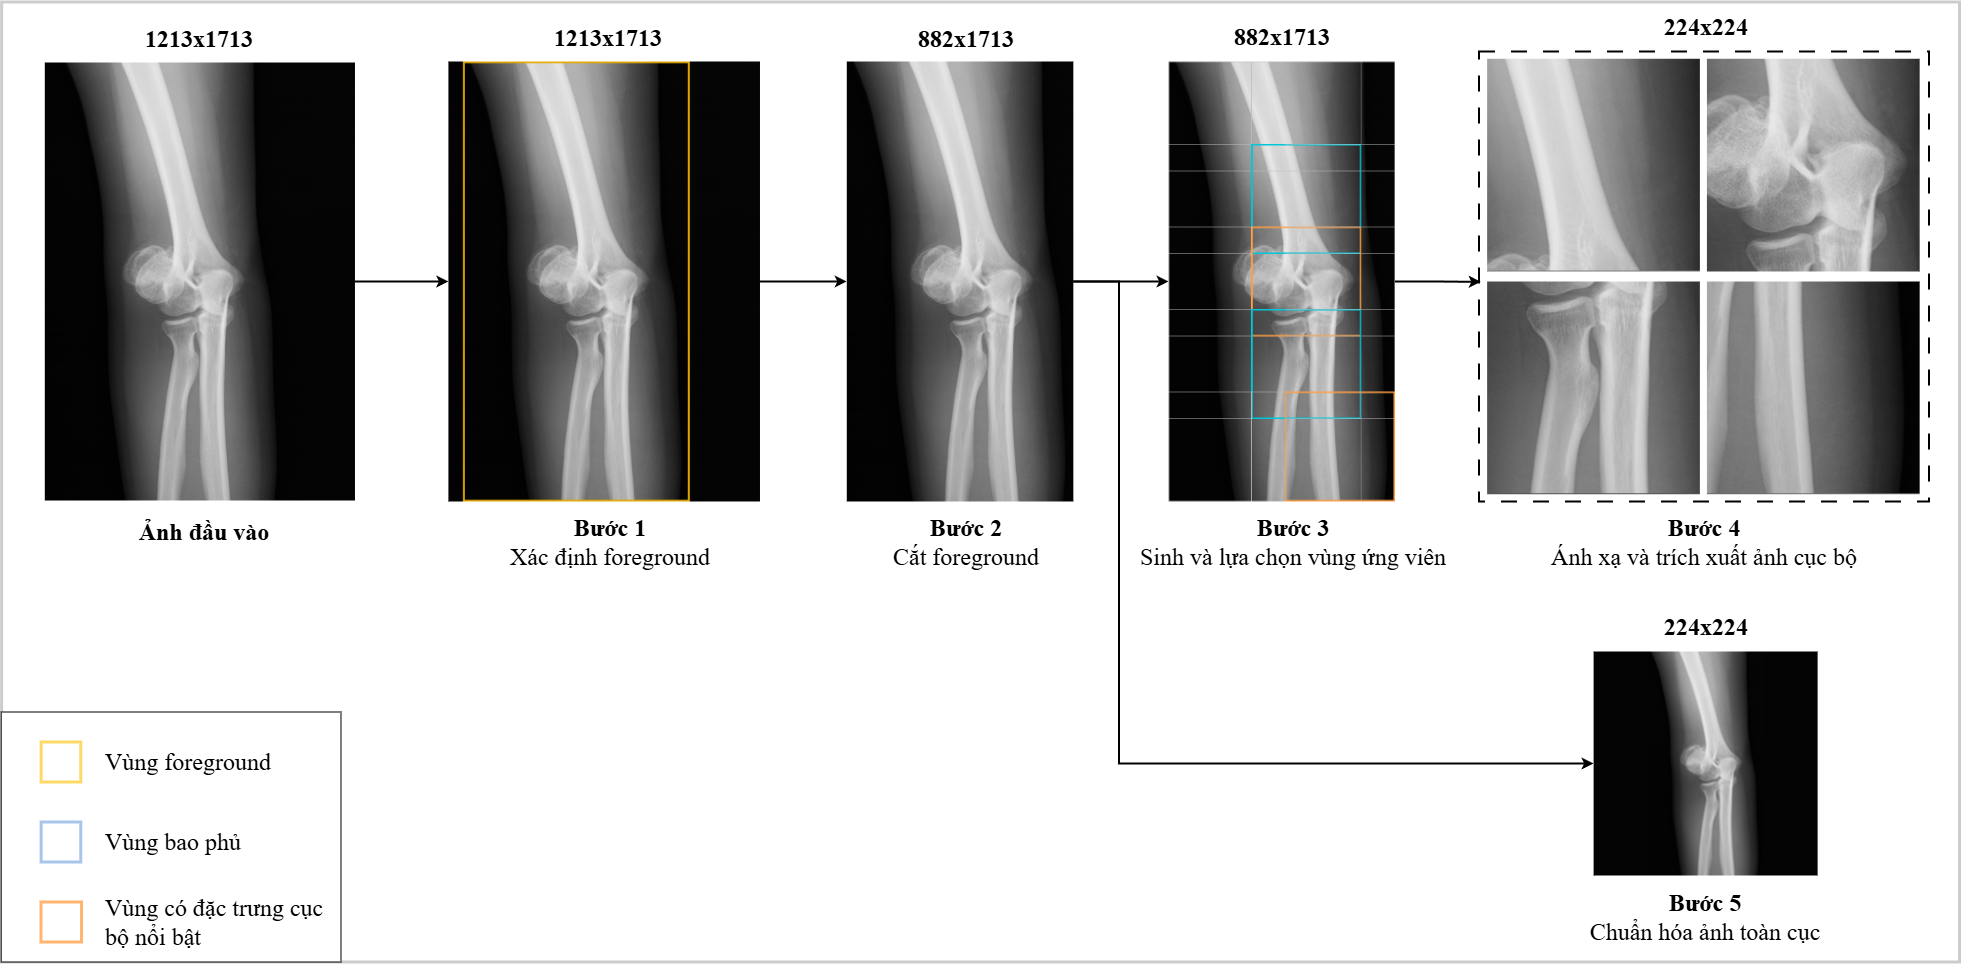
\includegraphics[width=\textwidth]{images/ImagePreprocess.png}
    \caption{Minh họa quy trình tạo ảnh toàn cục và các vùng ảnh cục bộ từ ảnh X-quang độ phân giải cao}
    \label{fig:ch3_high_resolution_preprocessing}
\end{figure}

Như minh họa trong Hình \ref{fig:ch3_high_resolution_preprocessing}, quy trình gồm xác định vùng tiền cảnh, cắt vùng nội dung, sinh và lựa chọn các cửa sổ ứng viên, ánh xạ các cửa sổ về ảnh nguồn, trích xuất bốn ảnh cục bộ và tạo ảnh toàn cục. Trước tiên, ảnh được chuyển sang thang xám và cường độ nền được ước lượng từ trung vị của dải điểm ảnh nằm dọc biên ảnh. 

\subsubsection{Xác định vùng tiền cảnh}
Một điểm ảnh được xem là thuộc vùng tiền cảnh khi độ lệch của nó so với mức nền vượt qua một ngưỡng thích nghi:

\begin{equation}M(p)=\mathbb{I}\left(\left|I(p)-\mu^{\partial}\right|\geq\tau\right),\qquad \tau=\max\left(\tau_{\min},4\sigma^{\partial}\right).\label{eq:ch3_foreground_mask}\end{equation}

Trong Công thức \ref{eq:ch3_foreground_mask}, $I(p)$ là cường độ tại vị trí $p$ của ảnh đang xử lý, $\mu^{\partial}$ là trung vị cường độ ở biên ảnh, $\sigma^{\partial}$ là độ lệch tuyệt đối trung vị đã hiệu chỉnh tại biên, $\tau_{\min}$ là mức tương phản tối thiểu, $\tau$ là ngưỡng thích nghi và $\mathbb{I}(\cdot)$ là hàm chỉ thị. Hình chữ nhật bao quanh các hàng và cột có tỷ lệ điểm ảnh tiền cảnh đủ lớn được mở rộng thêm một biên nhỏ để giảm nguy cơ cắt mất cấu trúc giải phẫu; nếu vùng ước lượng quá hẹp, quá nhỏ hoặc không giữ đủ năng lượng tương phản, toàn bộ ảnh $X$ được sử dụng thay cho phép cắt.

Từ vùng tiền cảnh, ảnh toàn cục được thay đổi kích thước theo cùng một tỷ lệ trên hai trục và được đệm thành ảnh vuông $224\times224$. Hệ số thay đổi kích thước được xác định bởi:

\begin{equation}s=\min\left(\frac{224}{W^{f}},\frac{224}{H^{f}}\right),\qquad X^{g}=\mathcal{L}_{224}\!\left(\mathcal{C}(X)\right).\label{eq:ch3_global_image}\end{equation}

Trong Công thức \ref{eq:ch3_global_image}, $W^{f}$ và $H^{f}$ lần lượt là chiều rộng và chiều cao của vùng tiền cảnh, $s$ là hệ số thay đổi kích thước, $\mathcal{C}(\cdot)$ là phép cắt vùng tiền cảnh và $\mathcal{L}_{224}(\cdot)$ là phép đổi kích thước giữ tỷ lệ kết hợp với đệm biên để thu được ảnh toàn cục $X^{g}$. Màu đệm được ước lượng từ trung vị biên của vùng ảnh thay vì gán cố định bằng màu đen, sau đó ảnh được chuẩn hóa theo quy tắc đầu vào của bộ mã hóa thị giác.

\subsubsection{Sinh và lựa chọn ứng viên}

Đối với nhánh cục bộ, cạnh dài của vùng tiền cảnh được đưa về tối đa $896$ điểm ảnh mà không phóng lớn ảnh có độ phân giải thấp. Trên ảnh trung gian này, các cửa sổ vuông $224\times224$ được sinh với bước dịch chuyển $168$ điểm ảnh; một cửa sổ được ưu tiên xem xét khi tỷ lệ điểm ảnh tiền cảnh bên trong không thấp hơn $0{,}60$. Tập cửa sổ ứng viên có thể được biểu diễn như sau:

\begin{equation}\mathcal{G}=\operatorname{Grid}\!\left(H^{c},W^{c};224,168\right),\qquad \mathcal{B}=\left\{b\in\mathcal{G}\mid r(b)\geq0{,}60\right\}.\label{eq:ch3_candidate_regions}\end{equation}

Trong Công thức \ref{eq:ch3_candidate_regions}, $H^{c}$ và $W^{c}$ là chiều cao và chiều rộng của ảnh trung gian, $\mathcal{G}$ là lưới các cửa sổ vuông cạnh $224$ được sinh với bước dịch chuyển $168$, $r(b)$ là tỷ lệ điểm ảnh tiền cảnh trong cửa sổ $b$, còn $\mathcal{B}$ là tập cửa sổ đáp ứng ngưỡng tiền cảnh; vị trí cuối mỗi trục được bổ sung khi cần thiết để hạn chế bỏ sót phần biên của vùng giải phẫu.

Mỗi cửa sổ ứng viên được chấm điểm từ ba thành phần gồm năng lượng Laplacian biểu thị mức thay đổi cường độ cục bộ, entropy biểu thị mức đa dạng của phân bố mức xám và tỷ lệ tiền cảnh biểu thị lượng nội dung khác nền:

\begin{equation}q(b)=0{,}55\,\widehat{E}(b)+0{,}35\,\widehat{\mathcal{H}}(b)+0{,}10\,r(b).\label{eq:ch3_candidate_score}\end{equation}

Trong Công thức \ref{eq:ch3_candidate_score}, $\widehat{E}(b)$ và $\widehat{\mathcal{H}}(b)$ lần lượt là năng lượng Laplacian và entropy của cửa sổ $b$ sau khi chuẩn hóa về đoạn $[0,1]$, $r(b)$ là tỷ lệ điểm ảnh tiền cảnh và $q(b)$ là điểm thông tin của cửa sổ. Trọng số lớn hơn dành cho năng lượng Laplacian làm điểm số nhạy hơn với biên và biến đổi kết cấu, trong khi entropy và tỷ lệ tiền cảnh cung cấp thêm thông tin về sự đa dạng cường độ và mức độ hiện diện của cấu trúc giải phẫu.

Việc chọn bốn vùng cục bộ được thực hiện theo hai vai trò. Hai vùng đầu tiên được chọn gần các vị trí phân bố đều dọc theo trục dài của vùng tiền cảnh nhằm duy trì độ bao phủ giải phẫu; với tâm cửa sổ đã chuẩn hóa, phép chọn vùng bao phủ thứ $j$ được mô tả bởi:

\begin{equation}b_{j}^{\mathrm{cov}}=\underset{b\in\mathcal{B}\setminus\mathcal{S}_{j}}{\operatorname{arg\,min}}\ \frac{\left\|\boldsymbol{c}(b)-\boldsymbol{t}_j\right\|_2}{0{,}5+0{,}5r(b)},\qquad j\in\{1,2\}.\label{eq:ch3_coverage_selection}\end{equation}

Trong Công thức \ref{eq:ch3_coverage_selection}, $b_{j}^{\mathrm{cov}}$ là vùng bao phủ thứ $j$, $\boldsymbol{c}(b)$ là tâm chuẩn hóa của cửa sổ $b$, $\boldsymbol{t}_j$ là vị trí bao phủ mục tiêu và $\mathcal{S}_{j}$ là tập vùng đã chọn trước bước thứ $j$. Thành phần ở mẫu số tạo ưu tiên nhẹ cho cửa sổ chứa nhiều tiền cảnh hơn khi khoảng cách đến vị trí mục tiêu tương đương.

Hai vùng còn lại ưu tiên các vị trí có điểm thông tin cao nhưng vẫn duy trì khoảng cách với các vùng đã chọn. Ở mỗi bước, các cửa sổ có mức chồng lấp lớn hơn $0{,}30$ với bất kỳ vùng đã chọn nào được loại khỏi tập xem xét, sau đó vùng tiêu điểm được xác định theo:

\begin{equation}b_{j}^{\mathrm{foc}}=\underset{b\in\mathcal{A}_{j}}{\operatorname{arg\,max}}\left[q(b)+0{,}35\min_{a\in\mathcal{S}_{j}}\left\|\boldsymbol{c}(b)-\boldsymbol{c}(a)\right\|_2\right],\qquad j\in\{1,2\}.\label{eq:ch3_focal_selection}\end{equation}

Trong Công thức \ref{eq:ch3_focal_selection}, $b_{j}^{\mathrm{foc}}$ là vùng tiêu điểm thứ $j$, $\mathcal{A}_{j}$ là tập cửa sổ còn hợp lệ tại bước chọn này và $\mathcal{S}_{j}$ là tập vùng đã được chọn. Số hạng thứ nhất ưu tiên vùng có biên và phân bố cường độ giàu thông tin, còn số hạng thứ hai hạn chế việc tập trung nhiều vùng tại cùng một vị trí; cách lựa chọn này tạo ra hai vùng bao phủ và hai vùng tiêu điểm với ngân sách tính toán cố định.

Khi mặt nạ tiền cảnh không tạo đủ số cửa sổ đạt ngưỡng, quy trình mở rộng việc xem xét sang toàn bộ cửa sổ đã sinh để hạn chế phụ thuộc vào một mặt nạ chưa ổn định. Nếu ràng buộc chồng lấp tiếp tục làm số vùng hợp lệ nhỏ hơn bốn, các vùng còn lại được bổ sung theo khoảng cách không gian và điểm thông tin; đối với ảnh quá nhỏ để tạo bốn cửa sổ phân biệt, một số vùng có thể được lặp lại theo thứ tự xác định nhằm duy trì kích thước đầu vào cố định mà không xem phần phóng lớn là thông tin mới.

\subsubsection{Ánh xạ về ảnh nguồn}

Các hộp được chọn trên ảnh trung gian được ánh xạ ngược về tọa độ của ảnh nguồn trước khi cắt, nhờ đó mỗi vùng cục bộ được lấy từ dữ liệu ảnh ban đầu thay vì từ ảnh trung gian đã thu nhỏ. Mỗi vùng sau đó được giữ tỷ lệ, đệm biên và chuẩn hóa thành ảnh $224\times224$:

\begin{equation}X_{m}^{\ell}=\mathcal{L}_{224}\!\left(X\!\mid_{b_m}\right),\qquad m=1,\ldots,4.\label{eq:ch3_local_images}\end{equation}

Trong Công thức \ref{eq:ch3_local_images}, $b_m$ là hộp thứ $m$ trên ảnh nguồn, $X\!\mid_{b_m}$ là vùng ảnh được cắt theo hộp này và $X_m^{\ell}$ là ảnh cục bộ tương ứng. Kết quả của quá trình xử lý một ảnh gồm ảnh toàn cục $X^{g}$, bốn ảnh cục bộ $\{X_m^{\ell}\}_{m=1}^{4}$ và tọa độ chuẩn hóa của bốn vùng; các thành phần này được tạo trước bộ mã hóa thị giác, vì vậy cơ chế độ phân giải cao được xem là một bước chuẩn bị đầu vào thay vì một bộ mã hóa độc lập.

\subsection{Bộ mã hóa thị giác}
\label{subsec:ch3_visual_encoder}

Bộ mã hóa thị giác của BiomedCLIP sử dụng kiến trúc Vision Transformer. Ảnh đầu vào được chia thành các mảnh ảnh, ánh xạ thành chuỗi biểu diễn và xử lý bằng các lớp Transformer. Ở mức khái quát, ảnh toàn cục được mã hóa như sau:

\begin{equation}
\boldsymbol{H}_{i}^{I}
=
\mathcal{E}_{I}\left(x_i^{img,g}\right),
\qquad
\boldsymbol{g}_{i}
=
\mathcal{P}_{I}\left(\boldsymbol{H}_{i,0}^{I}\right).
\label{eq:ch3_visual_encoder}
\end{equation}

Trong Công thức \ref{eq:ch3_visual_encoder}, $\mathcal{E}_{I}$ là bộ mã hóa thị giác, $\boldsymbol{H}_{i}^{I}$ là chuỗi đặc trưng ảnh, $\boldsymbol{H}_{i,0}^{I}$ là đặc trưng đại diện toàn cục, $\mathcal{P}_{I}$ là phép chiếu sang không gian chung và $\boldsymbol{g}_{i}\in\mathbb{R}^{D}$ là vectơ đặc trưng toàn cục.

Ảnh toàn cục và các vùng cục bộ dùng chung một bộ mã hóa thị giác. Nhờ chia sẻ trọng số, đặc trưng thu được nằm trong cùng một không gian:

\begin{equation}
\boldsymbol{\ell}_{i,m}
=
\mathcal{P}_{I}
\left(
\operatorname{Pool}
\left(
\mathcal{E}_{I}\left(x_{i,m}^{img,\ell}\right)
\right)
\right).
\label{eq:ch3_local_encoding}
\end{equation}

Trong Công thức \ref{eq:ch3_local_encoding}, $\operatorname{Pool}$ là phép gộp không gian dùng để tạo một số lượng hữu hạn đặc trưng cục bộ. Cấu hình thực nghiệm sử dụng một số lượng vùng cố định cho mỗi ảnh để chi phí tính toán giữa các mẫu không thay đổi. Mỗi vùng được tóm tắt bởi đặc trưng đại diện và các đặc trưng không gian đã gộp, thay vì giữ toàn bộ lưới mảnh ảnh của từng vùng.

Do các vùng cục bộ đến từ những vị trí khác nhau trên ảnh nguồn, tọa độ chuẩn hóa của mỗi vùng được chiếu thành biểu diễn vị trí và cộng vào đặc trưng nội dung:

\begin{equation}
\widetilde{\boldsymbol{\ell}}_{i,m}
=
\boldsymbol{\ell}_{i,m}
+
\mathcal{P}_{s}\left(\boldsymbol{b}_{i,m}\right),
\label{eq:ch3_spatial_encoding}
\end{equation}

trong đó $\boldsymbol{b}_{i,m}$ chứa tọa độ chuẩn hóa của vùng thứ $m$ và $\mathcal{P}_{s}$ là phép chiếu tọa độ. Cách biểu diễn này giúp mô hình phân biệt những vùng có nội dung gần giống nhau nhưng nằm ở các vị trí giải phẫu khác nhau.

Cuối cùng, nhánh ảnh tạo chuỗi đặc trưng gồm một phần tử toàn cục và các phần tử cục bộ:

\begin{equation}
\boldsymbol{V}_{i}
=
\left[
\boldsymbol{g}_{i};
\widetilde{\boldsymbol{\ell}}_{i,1};
\ldots;
\widetilde{\boldsymbol{\ell}}_{i,M}
\right]
\in
\mathbb{R}^{T_I\times D}.
\label{eq:ch3_visual_sequence}
\end{equation}

Chuỗi $\boldsymbol{V}_{i}$ vừa giữ bối cảnh toàn ảnh, vừa bảo toàn bằng chứng cục bộ cần thiết cho bước dung hợp với văn bản. Ký hiệu $T_I$ là tổng số phần tử trong chuỗi đặc trưng ảnh sau khi ghép. Khóa luận không đi sâu vào cấu trúc từng lớp bên trong bộ mã hóa vì thành phần này được kế thừa từ BiomedCLIP. Trọng tâm của phương pháp đề xuất nằm ở cách tạo đầu vào ảnh, thích nghi tham số và kết hợp các đặc trưng sau mã hóa.

\section{Nhánh biểu diễn văn bản}
\label{sec:ch3_text_branch}
Bổ sung cho các bằng chứng hình thái được trích xuất từ ảnh X-quang, nhánh biểu diễn văn bản có nhiệm vụ mã hóa thông tin lâm sàng $x_i^{txt}$ thành các đặc trưng ngữ cảnh theo từng token và một vectơ đại diện cho toàn bộ chuỗi. Trong khóa luận, nhánh này được kế thừa từ bộ mã hóa văn bản của BiomedCLIP \cite{BiomedCLIP}, với thành phần chính là PubMedBERT. Khác với các mô hình ngôn ngữ được tiền huấn luyện trên văn bản tổng quát, PubMedBERT được tiền huấn luyện từ đầu trên kho ngữ liệu y sinh và sử dụng bộ từ vựng được xây dựng trực tiếp từ miền dữ liệu này. Nhờ đó, mô hình phù hợp hơn với các thuật ngữ chuyên ngành xuất hiện trong thông tin lâm sàng.

\subsection{Tiền xử lý và mã hóa đầu vào}

Trước khi đưa vào PubMedBERT, chuỗi văn bản $x_i^{txt}$ được phân tách thành các đơn vị từ con bằng bộ mã hóa WordPiece tương ứng với mô hình. Hai token đặc biệt \texttt{[CLS]} và \texttt{[SEP]} lần lượt được thêm vào đầu và cuối chuỗi. Chuỗi sau khi mã hóa được cắt hoặc đệm đến độ dài tối đa $T_T=256$, tương ứng với cấu hình của BiomedCLIP:

\begin{equation}
\left(
\boldsymbol{u}_{i},
\boldsymbol{m}_{i}
\right)
=
\operatorname{Tokenizer}_{T}
\left(x_i^{txt}\right),
\label{eq:ch3_text_tokenization}
\end{equation}

trong đó $\boldsymbol{u}_{i}\in\mathbb{N}^{T_T}$ là chuỗi chỉ số token và $\boldsymbol{m}_{i}\in\{0,1\}^{T_T}$ là mặt nạ chú ý. Giá trị bằng $1$ trong $\boldsymbol{m}_{i}$ biểu thị một token hợp lệ, trong khi giá trị bằng $0$ biểu thị vị trí được thêm vào để đệm chuỗi.

\subsection{Bộ mã hóa văn bản}
\label{subsec:ch3_text_encoder}
Chuỗi chỉ số token và mặt nạ chú ý thu được ở bước trên tạo thành đầu vào trực tiếp của PubMedBERT. Từ các biểu diễn rời rạc này, bộ mã hóa tiếp tục xây dựng đặc trưng ngữ cảnh cho từng vị trí trong chuỗi. Trước khi đi qua các khối Transformer Encoder, mỗi token được ánh xạ thành một biểu diễn liên tục bằng tổng của embedding token, embedding vị trí và embedding phân đoạn:

\begin{equation}
\boldsymbol{H}_{i}^{T,(0)}
=
\boldsymbol{E}_{tok}\left(\boldsymbol{u}_{i}\right)
+
\boldsymbol{E}_{pos}
+
\boldsymbol{E}_{seg},
\label{eq:ch3_text_embedding}
\end{equation}

trong đó $\boldsymbol{H}_{i}^{T,(0)}\in\mathbb{R}^{T_T\times d_T}$ và $d_T=768$ là kích thước trạng thái ẩn của PubMedBERT. Trong trường hợp đầu vào chỉ gồm một chuỗi văn bản, các token sử dụng cùng một embedding phân đoạn.

PubMedBERT được xây dựng theo kiến trúc BERT-base, bao gồm $L_T=12$ khối Transformer Encoder. Mỗi khối gồm một lớp chú ý self-attention đa đầu và một mạng truyền thẳng theo từng vị trí. Tại khối thứ $\ell$, quá trình cập nhật biểu diễn có thể được khái quát như sau:

\begin{align}
\widetilde{\boldsymbol{H}}_{i}^{T,(\ell)}
&=
\operatorname{LayerNorm}
\left(
\boldsymbol{H}_{i}^{T,(\ell-1)}
+
\operatorname{MHSA}
\left(
\boldsymbol{H}_{i}^{T,(\ell-1)},
\boldsymbol{m}_{i}
\right)
\right),
\\
\boldsymbol{H}_{i}^{T,(\ell)}
&=
\operatorname{LayerNorm}
\left(
\widetilde{\boldsymbol{H}}_{i}^{T,(\ell)}
+
\operatorname{FFN}
\left(
\widetilde{\boldsymbol{H}}_{i}^{T,(\ell)}
\right)
\right),
\label{eq:ch3_text_transformer}
\end{align}

với $\ell=1,\ldots,L_T$. Cơ chế self-attention hai chiều cho phép biểu diễn tại mỗi vị trí được xác định dựa trên toàn bộ ngữ cảnh của chuỗi. Mặt nạ $\boldsymbol{m}_{i}$ được sử dụng để loại bỏ ảnh hưởng của các token đệm trong quá trình tính toán chú ý.

Sau khối Transformer cuối cùng, PubMedBERT tạo ra ma trận đặc trưng ngữ cảnh:

\begin{equation}
\boldsymbol{H}_{i}^{T}
=
TextEncoder
\left(
\boldsymbol{u}_{i},
\boldsymbol{m}_{i}
\right)
=
\boldsymbol{H}_{i}^{T,(L_T)}
\in
\mathbb{R}^{T_T\times d_T}.
\label{eq:ch3_text_contextual_features}
\end{equation}

Mỗi hàng của $\boldsymbol{H}_{i}^{T}$ là biểu diễn ngữ cảnh của một token. Trong đó, vector tại vị trí đầu tiên, tương ứng với token \texttt{[CLS]}, được sử dụng làm biểu diễn tổng hợp của toàn bộ chuỗi:

\begin{equation}
\boldsymbol{h}_{i}^{T}
=
\boldsymbol{H}_{i,0}^{T}
\in
\mathbb{R}^{d_T}.
\label{eq:ch3_text_cls}
\end{equation}

Theo kiến trúc BiomedCLIP, biểu diễn \texttt{[CLS]} tiếp tục được đưa qua bộ chiếu văn bản $\mathcal{P}_{T}$, được hiện thực bằng một mạng MLP. Phép chiếu chuyển đặc trưng từ không gian ẩn của PubMedBERT sang không gian nhúng có kích thước $D=512$:

\begin{equation}
\boldsymbol{t}_{i}
=
\operatorname{Norm}_{2}
\left(
\mathcal{P}_{T}
\left(
\boldsymbol{h}_{i}^{T}
\right)
\right)
\in
\mathbb{R}^{D}.
\label{eq:ch3_global_text}
\end{equation}

Kết quả cuối cùng của nhánh biểu diễn văn bản là vector $\boldsymbol{t}_{i}$ đã được chuẩn hóa theo chuẩn $L_2$. Vector này mang thông tin ngữ nghĩa tổng quát của nội dung lâm sàng và có cùng kích thước với không gian biểu diễn được định nghĩa trong BiomedCLIP.

Kết thúc hai nhánh mã hóa, mỗi mẫu được biểu diễn bởi chuỗi đặc trưng ảnh $\boldsymbol{V}_{i}$, ma trận đặc trưng văn bản $\boldsymbol{H}_{i}^{T}$ và các vectơ toàn cục tương ứng. Mặc dù các biểu diễn này kế thừa tri thức y sinh từ BiomedCLIP, sự khác biệt giữa dữ liệu tiền huấn luyện và dữ liệu X-quang xương đích vẫn đòi hỏi hai bộ mã hóa được thích nghi trước khi thực hiện dung hợp.

\section{Thích nghi tham số bằng LoRA}
\label{sec:ch3_lora}

Hai bộ mã hóa đã được tiền huấn luyện trên dữ liệu y sinh quy mô lớn, nhưng dữ liệu X-quang xương đích vẫn có khác biệt về phân bố ảnh, cách ghi bệnh sử và hệ thống nhãn. Việc tinh chỉnh toàn bộ tham số có chi phí lớn và dễ quá khớp khi dữ liệu gán nhãn hạn chế. XBone-Net vì vậy sử dụng LoRA để học phần cập nhật hạng thấp cho các phép biến đổi tuyến tính quan trọng.

Với ma trận trọng số nền $\boldsymbol{W}\in\mathbb{R}^{d_o\times d_i}$, LoRA biểu diễn ma trận sau thích nghi theo công thức chuẩn:

\begin{equation}
\boldsymbol{W}'
=
\boldsymbol{W}
+
\frac{\alpha}{r}
\boldsymbol{B}\boldsymbol{A},
\qquad
\boldsymbol{A}\in\mathbb{R}^{r\times d_i},
\quad
\boldsymbol{B}\in\mathbb{R}^{d_o\times r},
\quad
r\ll\min(d_i,d_o).
\label{eq:ch3_lora}
\end{equation}

Trong Công thức \ref{eq:ch3_lora}, $\boldsymbol{W}$ được giữ cố định, $\boldsymbol{A}$ và $\boldsymbol{B}$ là hai ma trận được cập nhật, $r$ là hạng thích nghi và $\alpha$ là hệ số tỷ lệ. Nhờ đó, mô hình chỉ học một phần nhỏ tham số bổ sung nhưng vẫn có thể điều chỉnh cả biểu diễn ảnh lẫn biểu diễn văn bản cho miền dữ liệu mới. Khi triển khai, phần cập nhật có thể được giữ riêng hoặc gộp tương đương vào trọng số nền mà không làm thay đổi kết quả tính toán.

LoRA chỉ điều chỉnh cách từng bộ mã hóa biểu diễn dữ liệu trong miền đích; bản thân kỹ thuật này chưa thực hiện trao đổi thông tin giữa ảnh và văn bản. Sau khi hai nhánh đã tạo ra các đặc trưng thích nghi, các biểu diễn này được chuyển đến mô-đun dung hợp để mô hình hóa quan hệ giữa dấu hiệu thị giác và ngữ cảnh lâm sàng.

\section{Dung hợp đa phương thức bằng chú ý chéo}
\label{sec:ch3_fusion}

Từ hai nhánh mã hóa, hệ thống thu được chuỗi đặc trưng ảnh $\boldsymbol{V}_{i}$, ma trận đặc trưng văn bản $\boldsymbol{H}_{i}^{T}$ và hai biểu diễn toàn cục $\boldsymbol{g}_{i}$, $\boldsymbol{t}_{i}$. Nếu chỉ ghép nối trực tiếp các vectơ toàn cục, mô hình chưa thể hiện rõ nội dung lâm sàng nào liên quan đến từng dấu hiệu trên ảnh. Vì vậy, XBone-Net sử dụng cơ chế chú ý chéo hai chiều để mỗi phương thức chủ động truy vấn thông tin cần thiết từ phương thức còn lại trước khi hình thành biểu diễn chung.

\begin{figure}[H]
    \centering
    
\includegraphics[width=0.62\textwidth]{images/fusion.png}
    \caption{Mô-đun dung hợp bằng chú ý chéo hai chiều}
    \label{fig:ch3_fusion}
\end{figure}

Với chuỗi truy vấn $\boldsymbol{X}$ và chuỗi cung cấp ngữ cảnh $\boldsymbol{Y}$, phép chú ý chéo nhiều đầu được xây dựng từ ba phép chiếu chuẩn:

\begin{equation}
\boldsymbol{Q}
=
\boldsymbol{X}\boldsymbol{W}_{Q},
\qquad
\boldsymbol{K}
=
\boldsymbol{Y}\boldsymbol{W}_{K},
\qquad
\boldsymbol{U}
=
\boldsymbol{Y}\boldsymbol{W}_{V}.
\label{eq:ch3_qkv}
\end{equation}

Đầu ra chú ý được tính bởi:

\begin{equation}
\operatorname{Attention}
\left(
\boldsymbol{Q},
\boldsymbol{K},
\boldsymbol{U}
\right)
=
\operatorname{Softmax}
\left(
\frac{
\boldsymbol{Q}\boldsymbol{K}^{\mathsf{T}}
}{
\sqrt{d_h}
}
\right)
\boldsymbol{U},
\label{eq:ch3_attention}
\end{equation}

trong đó $d_h$ là số chiều của mỗi đầu chú ý. Mặt nạ được áp dụng trước hàm Softmax để loại bỏ các vị trí đệm của chuỗi văn bản hoặc các vùng ảnh không hợp lệ.

Ở chiều thứ nhất, đặc trưng ảnh toàn cục đóng vai trò truy vấn, còn các đặc trưng văn bản cung cấp khóa và giá trị. Kết quả là biểu diễn ảnh đã được bổ sung ngữ cảnh lâm sàng:

\begin{equation}
\boldsymbol{h}_{i}^{I}
=
\operatorname{LN}
\left(
\boldsymbol{g}_{i}
+
\operatorname{Attention}
\left(
\boldsymbol{g}_{i},
\boldsymbol{H}_{i}^{T},
\boldsymbol{H}_{i}^{T}
\right)
\right).
\label{eq:ch3_image_from_text}
\end{equation}

Ở chiều ngược lại, đặc trưng văn bản toàn cục truy vấn chuỗi đặc trưng ảnh để thu nhận bằng chứng thị giác phù hợp:

\begin{equation}
\boldsymbol{h}_{i}^{T}
=
\operatorname{LN}
\left(
\boldsymbol{t}_{i}
+
\operatorname{Attention}
\left(
\boldsymbol{t}_{i},
\boldsymbol{V}_{i},
\boldsymbol{V}_{i}
\right)
\right).
\label{eq:ch3_text_from_image}
\end{equation}

Hai biểu diễn sau chú ý được ghép và đưa qua một perceptron đa tầng để tạo vectơ đặc trưng tổng hợp:

\begin{equation}
\boldsymbol{z}_{i}
=
\operatorname{LN}
\left(
\operatorname{MLP}
\left(
\left[
\boldsymbol{h}_{i}^{I};
\boldsymbol{h}_{i}^{T}
\right]
\right)
\right)
\in
\mathbb{R}^{D}.
\label{eq:ch3_fused_representation}
\end{equation}

Hình \ref{fig:ch3_fusion} cho thấy hai hướng chú ý được thực hiện song song. Kết nối phần dư và chuẩn hóa lớp giúp giữ lại đặc trưng ban đầu, trong khi perceptron đa tầng học cách tổng hợp hai biểu diễn đã được bổ sung ngữ cảnh.

Kết quả của quá trình trên là vectơ đa phương thức $\boldsymbol{z}_{i}$, trong đó thông tin ảnh và văn bản đã được tổng hợp trong cùng một biểu diễn. Vectơ này là đầu vào trực tiếp của bộ phân loại, do đó quyết định cuối cùng không còn dựa trên từng phương thức riêng lẻ mà dựa trên quan hệ đã học giữa chúng.

\section{Bộ phân loại bằng mạng nguyên mẫu}
\label{sec:ch3_prototype}

Trên không gian đặc trưng đa phương thức được tạo bởi mô-đun dung hợp, XBone-Net thực hiện phân loại theo nguyên lý của mạng nguyên mẫu \cite{Snell2017ProtoNet}. Thay vì sử dụng một lớp tuyến tính với trọng số lớp được học trực tiếp, mỗi lớp được biểu diễn bằng tâm của các vectơ $\boldsymbol{z}_{i}$ thuộc lớp tương ứng. Cách xây dựng này cho phép diễn giải dự đoán thông qua mức độ gần giữa mẫu và từng tâm lớp, đồng thời tạo ra một không gian khoảng cách có thể tiếp tục được khai thác trong bước phát hiện OOD.

\begin{figure}[H]
    \centering
    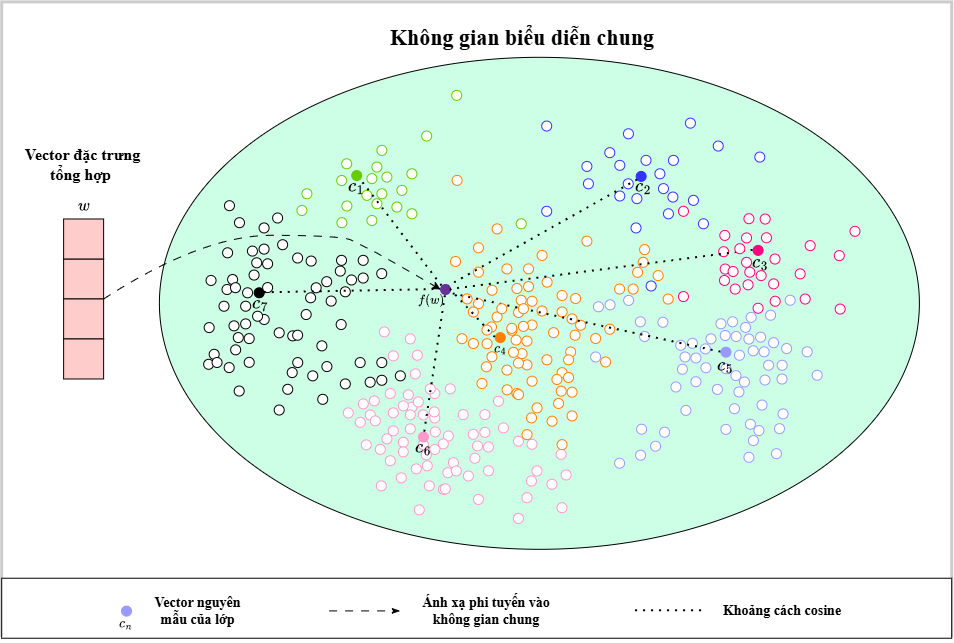
\includegraphics[width=0.92\textwidth]{images/protonet.png}
    \caption{Phân loại vectơ đặc trưng tổng hợp trong không gian nguyên mẫu}
    \label{fig:ch3_prototype}
\end{figure}

Với $\mathcal{I}_{k}=\left\{i\mid y_i=y_k\right\}$ là tập chỉ số các mẫu huấn luyện thuộc lớp $y_k$, nguyên mẫu lớp được ước lượng bằng trung bình đặc trưng:

\begin{equation}
\boldsymbol{c}_{k}
=
\frac{1}{\left|\mathcal{I}_{k}\right|}
\sum_{i\in\mathcal{I}_{k}}
\boldsymbol{z}_{i}.
\label{eq:ch3_prototype}
\end{equation}

Khoảng cách giữa mẫu mới và nguyên mẫu có thể được xây dựng từ độ tương đồng côsin:

\begin{equation}
d
\left(
\boldsymbol{z}_{i},
\boldsymbol{c}_{k}
\right)
=
1
-
\frac{
\boldsymbol{z}_{i}^{\mathsf{T}}\boldsymbol{c}_{k}
}{
\left\|\boldsymbol{z}_{i}\right\|_{2}
\left\|\boldsymbol{c}_{k}\right\|_{2}
}.
\label{eq:ch3_cosine_distance}
\end{equation}

Xác suất dự đoán được tính theo phân phối Softmax trên khoảng cách âm:

\begin{equation}
p
\left(
y_k\mid\boldsymbol{z}_{i}
\right)
=
\frac{
\exp
\left(
-d\left(\boldsymbol{z}_{i},\boldsymbol{c}_{k}\right)/\tau_c
\right)
}{
\sum_{j=1}^{K}
\exp
\left(
-d\left(\boldsymbol{z}_{i},\boldsymbol{c}_{j}\right)/\tau_c
\right)
},
\label{eq:ch3_prototype_probability}
\end{equation}

trong đó $\tau_c$ là hệ số nhiệt độ. Nhãn dự đoán là lớp có xác suất lớn nhất, tương đương với lớp có nguyên mẫu gần nhất theo độ đo đã chọn. Các nguyên mẫu là thống kê của tập huấn luyện, không phải tham số nhận đạo hàm. Khi biểu diễn thay đổi trong quá trình huấn luyện, các tâm lớp được ước lượng lại từ tập huấn luyện trước bước đánh giá.

Các phần trên xác định luồng truyền thuận của XBone-Net từ dữ liệu đầu vào đến xác suất phân loại. Tuy nhiên, các thành phần không được tối ưu đồng thời ngay từ đầu, bởi việc thích nghi không gian ảnh-văn bản và việc học nhiệm vụ phân loại có mục tiêu khác nhau. Vì vậy, quá trình huấn luyện được tách thành hai giai đoạn ngoại tuyến.

\section{Huấn luyện hai giai đoạn trong quá trình ngoại tuyến}
\label{sec:ch3_offline_training}
Quy trình ngoại tuyến lần lượt giải quyết hai yêu cầu của hệ thống. Giai đoạn thứ nhất điều chỉnh các bộ mã hóa để ảnh X-quang và thông tin lâm sàng tương ứng được biểu diễn phù hợp hơn trong miền dữ liệu đích. Trên nền không gian đã thích nghi, giai đoạn thứ hai học tương tác liên phương thức và tối ưu quyết định phân loại có xét đến sự mất cân bằng giữa các lớp.

\subsection{Giai đoạn 1: thích nghi miền bằng khớp ngữ nghĩa}
\label{subsec:ch3_phase1}

\begin{figure}[htbp]
    \centering
    
\includegraphics[width=0.84\textwidth]{images/domain.png}
    \caption{Giai đoạn thích nghi miền bằng khớp ngữ nghĩa ảnh-văn bản}
    \label{fig:ch3_phase1}
\end{figure}

Giai đoạn thứ nhất được minh họa trong Hình \ref{fig:ch3_phase1}. Ảnh X-quang và thông tin lâm sàng tương ứng được đưa qua hai bộ mã hóa để tạo các vectơ trong cùng một không gian. Các trọng số nền của BiomedCLIP được đóng băng, còn các ma trận LoRA và thành phần tổng hợp đặc trưng ảnh cục bộ được cập nhật. Mô-đun dung hợp và mạng nguyên mẫu chưa tham gia vào mục tiêu tối ưu ở giai đoạn này.

Giai đoạn này sử dụng hàm mất mát khớp ngữ nghĩa (Semantic Matching Loss) với phân phối đích mềm theo nhãn lớp. Trước hết, độ tương đồng giữa ảnh thứ $i$ và văn bản thứ $j$ được tính bằng độ tương đồng côsin có điều chỉnh nhiệt độ:

\begin{equation}
s_{ij}
=
\frac{
\overline{\boldsymbol{v}}_{i}^{\mathsf{T}}
\overline{\boldsymbol{t}}_{j}
}{
\tau_{\mathrm{SM}}
},
\label{eq:ch3_contrastive_similarity}
\end{equation}

trong đó $\overline{\boldsymbol{v}}_{i}$ và $\overline{\boldsymbol{t}}_{j}$ là các vectơ đã chuẩn hóa, còn $\tau_{\mathrm{SM}}$ là hệ số nhiệt độ. Biểu diễn ảnh dùng cho giai đoạn này lấy đặc trưng toàn cục làm điểm tựa và bổ sung tóm tắt có trọng số của các vùng cục bộ.

Với một lô gồm $B$ cặp ảnh-văn bản, trọng số đích mềm chưa chuẩn hóa được xác định theo quan hệ ngữ nghĩa giữa các cặp:

\begin{equation}
\widetilde{q}_{ij}
=
\mathbf{1}\left[i=j\right]
+
\rho\,
\mathbf{1}\left[i\neq j\right]
\mathbf{1}\left[y_i=y_j\right],
\qquad
0\leq\rho\leq 1.
\label{eq:ch3_semantic_target}
\end{equation}

Trong Công thức \ref{eq:ch3_semantic_target}, cặp ảnh-văn bản đúng của cùng một mẫu nhận trọng số lớn nhất, các cặp khác nhưng cùng nhãn nhận trọng số mềm $\rho$, còn các cặp khác lớp nhận trọng số bằng không. Các phân phối đích theo hai chiều được chuẩn hóa lần lượt theo hàng và theo cột:

\begin{equation}
\begin{aligned}
q_{ij}^{I\rightarrow T}
&=
\frac{\widetilde{q}_{ij}}
{\sum_{n=1}^{B}\widetilde{q}_{in}},
&
q_{ji}^{T\rightarrow I}
&=
\frac{\widetilde{q}_{ij}}
{\sum_{n=1}^{B}\widetilde{q}_{nj}}.
\end{aligned}
\label{eq:ch3_semantic_target_normalization}
\end{equation}

Từ các điểm tương đồng, mô hình tạo hai phân phối dự đoán:

\begin{equation}
\begin{aligned}
p_{ij}^{I\rightarrow T}
&=
\frac{\exp\left(s_{ij}\right)}
{\sum_{n=1}^{B}\exp\left(s_{in}\right)},
&
p_{ji}^{T\rightarrow I}
&=
\frac{\exp\left(s_{ij}\right)}
{\sum_{n=1}^{B}\exp\left(s_{nj}\right)}.
\end{aligned}
\label{eq:ch3_semantic_predictions}
\end{equation}

Hàm mất mát khớp ngữ nghĩa là trung bình của entropy chéo đích mềm theo hai chiều:

\begin{equation}
\mathcal{L}_{\mathrm{SM}}
=
-
\frac{1}{2B}
\sum_{i=1}^{B}
\sum_{j=1}^{B}
\left[
q_{ij}^{I\rightarrow T}
\log p_{ij}^{I\rightarrow T}
+
q_{ji}^{T\rightarrow I}
\log p_{ji}^{T\rightarrow I}
\right].
\label{eq:ch3_phase1_loss}
\end{equation}

Dạng mất mát trong Công thức \ref{eq:ch3_phase1_loss} kế thừa nguyên lý khớp ngữ nghĩa hai chiều của các mô hình ảnh-văn bản y khoa \cite{MedCLIP}. So với nhãn khớp cứng, phân phối đích mềm tránh xem mọi cặp khác mẫu là âm hoàn toàn khi chúng cùng mô tả một lớp bệnh. Việc lấy mẫu theo lớp làm tăng khả năng một lô có nhiều cặp cùng lớp để cung cấp tín hiệu ngữ nghĩa cho mục tiêu này.

Sau giai đoạn này, hai bộ mã hóa đã được điều chỉnh để tạo ra không gian ảnh--văn bản phù hợp hơn với dữ liệu X-quang xương. Tuy nhiên, các đặc trưng mới chỉ được căn chỉnh ở mức biểu diễn và chưa được tối ưu trực tiếp cho quyết định phân loại đa lớp. Vì vậy, giai đoạn thứ hai tiếp tục sử dụng các bộ mã hóa đã thích nghi, đồng thời đưa mô-đun dung hợp và mạng nguyên mẫu vào quá trình huấn luyện có giám sát.

\subsection{Giai đoạn 2: học dung hợp và phân loại}
\label{subsec:ch3_phase2}

\begin{figure}[htbp]
    \centering
    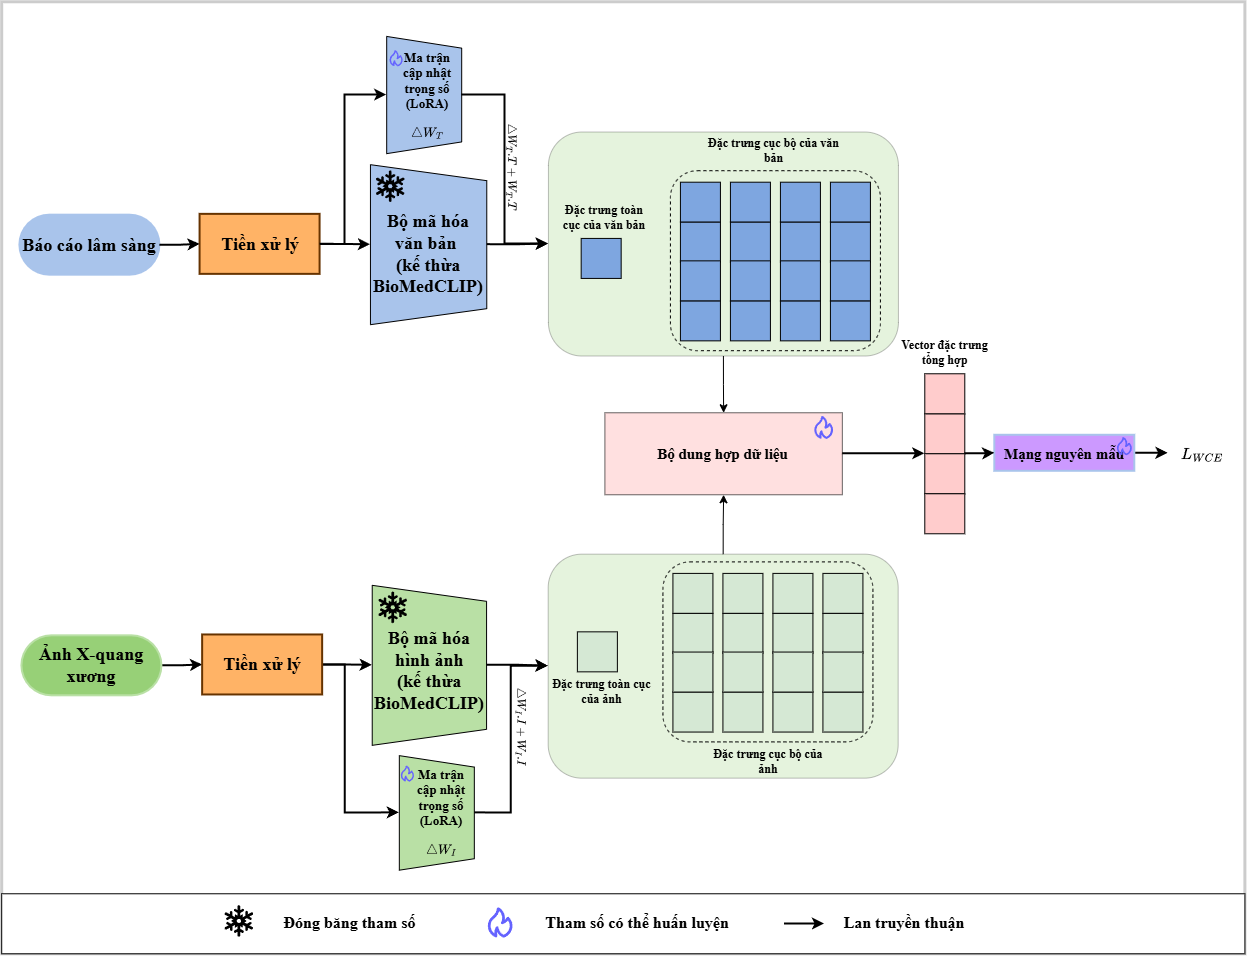
\includegraphics[width=0.90\textwidth]{images/classification.png}
    \caption{Giai đoạn học dung hợp và phân loại bằng mạng nguyên mẫu}
    \label{fig:ch3_phase2}
\end{figure}

Trong giai đoạn thứ hai, hai nhánh mã hóa tạo chuỗi đặc trưng toàn cục và cục bộ. Các chuỗi này được đưa qua mô-đun chú ý chéo để tạo vectơ tổng hợp $\boldsymbol{z}_{i}$. Mạng nguyên mẫu sử dụng các vectơ của tập huấn luyện để ước lượng tâm lớp và tính xác suất dự đoán. Trọng số nền của BiomedCLIP tiếp tục được giữ cố định, trong khi LoRA, thành phần biểu diễn ảnh cục bộ và mô-đun dung hợp được cập nhật.

Do số mẫu của các lớp có thể chênh lệch lớn, hàm mất mát sử dụng trọng số cân bằng lớp dựa trên số lượng mẫu hiệu dụng \cite{Cui2019ClassBalanced}. Với $n_k$ là số mẫu của lớp $k$, trọng số chưa chuẩn hóa được xác định bởi:

\begin{equation}
w_k
\propto
\frac{1-\beta}{1-\beta^{n_k}},
\qquad
0\leq\beta<1.
\label{eq:ch3_class_weight}
\end{equation}

Sau khi chuẩn hóa các trọng số để giữ thang đo ổn định, mục tiêu phân loại là entropy chéo có trọng số:

\begin{equation}
\mathcal{L}_{\mathrm{P2}}
=
-
\frac{1}{B}
\sum_{i=1}^{B}
w_{y_i}
\log
p
\left(
y=y_i
\mid
\boldsymbol{z}_{i}
\right).
\label{eq:ch3_phase2_loss}
\end{equation}

Sau mỗi chu kỳ huấn luyện, các nguyên mẫu được ước lượng lại bằng trạng thái hiện tại của mô hình trên tập huấn luyện, sau đó mới đánh giá trên tập kiểm định. Trạng thái mô hình tốt nhất được lựa chọn theo độ đo đã xác định trước trên tập kiểm định. Cuối cùng, các nguyên mẫu được tính lại từ tập huấn luyện bằng trạng thái đã chọn. Tập kiểm thử không được dùng để cập nhật tham số, ước lượng tâm lớp hoặc lựa chọn mô hình.

Kết quả của quá trình ngoại tuyến là tập tham số LoRA, mô-đun dung hợp, trạng thái bộ mã hóa và các tâm lớp đã được xác định từ dữ liệu huấn luyện. Các thành phần này được cố định và chuyển sang quy trình trực tuyến để xử lý từng ca mới mà không thực hiện thêm bất kỳ bước cập nhật nào.

\section{Suy luận trong quá trình trực tuyến}
\label{sec:ch3_online_inference}

\begin{figure}[H]
    \centering
    
\includegraphics[width=\textwidth]{images/online.png}
    \caption{Quy trình suy luận trực tuyến và phát hiện mẫu ngoài phân phối}
    \label{fig:ch3_online}
\end{figure}

Khi tiếp nhận một ca mới, ảnh X-quang và thông tin lâm sàng được xử lý bằng đúng các phép biến đổi đã sử dụng trong huấn luyện. Hai bộ mã hóa tạo đặc trưng ảnh và văn bản, mô-đun chú ý chéo tạo vectơ tổng hợp, sau đó mạng nguyên mẫu tính xác suất cho từng lớp. Toàn bộ tham số LoRA, mô-đun dung hợp và các nguyên mẫu lớp đều được cố định. Quá trình này không tính đạo hàm và không cập nhật tâm lớp từ mẫu mới. Kết quả trên cho biết lớp nào gần mẫu nhất trong số các lớp đã biết, nhưng chưa cho biết mẫu có thực sự phù hợp với phân bố huấn luyện hay không. 

Vì vậy, ngoài kết quả phân loại, hệ thống hỗ trợ một mô-đun hậu xử lý để phát hiện mẫu ngoài phân phối dựa theo khoảng cách, với độ đo phổ biến là khoảng cách Mahalanobis từ biểu diễn tổng hợp đến lớp gần nhất \cite{Lee2018MahalanobisOOD}:

\begin{equation}
s_{\mathrm{OOD}}
\left(x^{img},x^{txt}\right)
=
\min_{k}
\left(
\boldsymbol{z}-\boldsymbol{\mu}_{k}
\right)^{\mathsf{T}}
\boldsymbol{\Sigma}^{-1}
\left(
\boldsymbol{z}-\boldsymbol{\mu}_{k}
\right),
\label{eq:ch3_ood_score}
\end{equation}

trong đó $\boldsymbol{\mu}_{k}$ là tâm đặc trưng của lớp $k$ và $\boldsymbol{\Sigma}$ là ma trận hiệp phương sai được ước lượng từ dữ liệu trong phân phối, còn $\boldsymbol{z}$ là biểu diễn tổng hợp của $x^{img}$ và $x^{txt}$. Ngưỡng $\tau$ được hiệu chỉnh chỉ bằng dữ liệu huấn luyện và kiểm định. Thống nhất với ký hiệu ở Chương 1, quy tắc đầu ra của hệ thống là:

\begin{equation}
\widehat{y}
=
\begin{cases}
\mathrm{OOD},
& \text{nếu }s_{\mathrm{OOD}}\left(x^{img},x^{txt}\right)>\tau,\\[4pt]
\displaystyle
\operatorname*{arg\,max}_{y_k\in\mathcal{Y}}
p\left(y_k\mid x^{img},x^{txt}\right),
& \text{ngược lại}.
\end{cases}
\label{eq:ch3_ood_decision}
\end{equation}

Mô-đun phát hiện ngoài phân phối không thay đổi dự đoán nội tại của XBone-Net. Nó cung cấp thêm một tín hiệu cảnh báo về mức độ phù hợp của mẫu với phân bố đã quan sát. Vì vậy, đầu ra phân loại và cảnh báo ngoài phân phối có hai vai trò khác nhau: đầu ra thứ nhất chọn lớp gần nhất trong tập lớp đã biết, còn đầu ra thứ hai đánh giá liệu quyết định đó có được thực hiện trên một mẫu đủ quen thuộc hay không.

\section{Tóm tắt chương}

Chương này đã trình bày XBone-Net theo luồng từ tổng quan đến từng thành phần. Nhánh ảnh sử dụng bộ mã hóa thị giác kế thừa từ BiomedCLIP và cơ chế xử lý độ phân giải cao để kết hợp bối cảnh toàn cục với chi tiết cục bộ. Nhánh văn bản mã hóa thông tin lâm sàng trong cùng không gian đặc trưng. LoRA thích nghi hai bộ mã hóa với số tham số huấn luyện nhỏ, cơ chế chú ý chéo hai chiều trao đổi thông tin giữa hai phương thức và mạng nguyên mẫu thực hiện quyết định theo khoảng cách đến tâm lớp.

Quy trình huấn luyện gồm hai giai đoạn ngoại tuyến. Giai đoạn thứ nhất căn chỉnh biểu diễn ảnh-văn bản bằng hàm mất mát khớp ngữ nghĩa, còn giai đoạn thứ hai tối ưu biểu diễn dung hợp và mục tiêu phân loại có cân bằng lớp. Trong quá trình trực tuyến, mô hình giữ cố định toàn bộ tham số, thực hiện phân loại cho ca mới và có thể bổ sung cảnh báo ngoài phân phối đã được hiệu chỉnh trước.
